Given the restricted execution domain of PaaS clouds, we believe that it is possible
to design a system that predicts response time SLAs for PaaS-hosted web APIs using only
static information from the web API code itself.  To enable this, we design Cerebro
with three primary components:
\begin{itemize}
\item A static analysis tool that extracts the longest sequence of cloud SDK operations invoked by a web API code across paths in a method (web API operation),
\item A monitoring agent that runs in the target cloud platform that efficiently profiles the performance of the underlying cloud SDK operations (which we will call Watchtower), and
\item A prediction mechanism that uses the outputs of these two components to accurately predict an upper bound on the execution time of the web API (which we call the SLA predictor).
\end{itemize}
In our prototype, we perform Cerebro analysis at deployment time of a web API.  That is,
when a developer uploads their application to the cloud platform, Cerebro performs
the static analysis on the web API and requests a prediction for the longest path (currently
number and type of SDK operations) for each web API operation from the SLA predictor.
The SLA predictor accesses the time series data from Watchtower to produce an 
SLA prediction for each operation.

%\begin{figure}
%\centering
%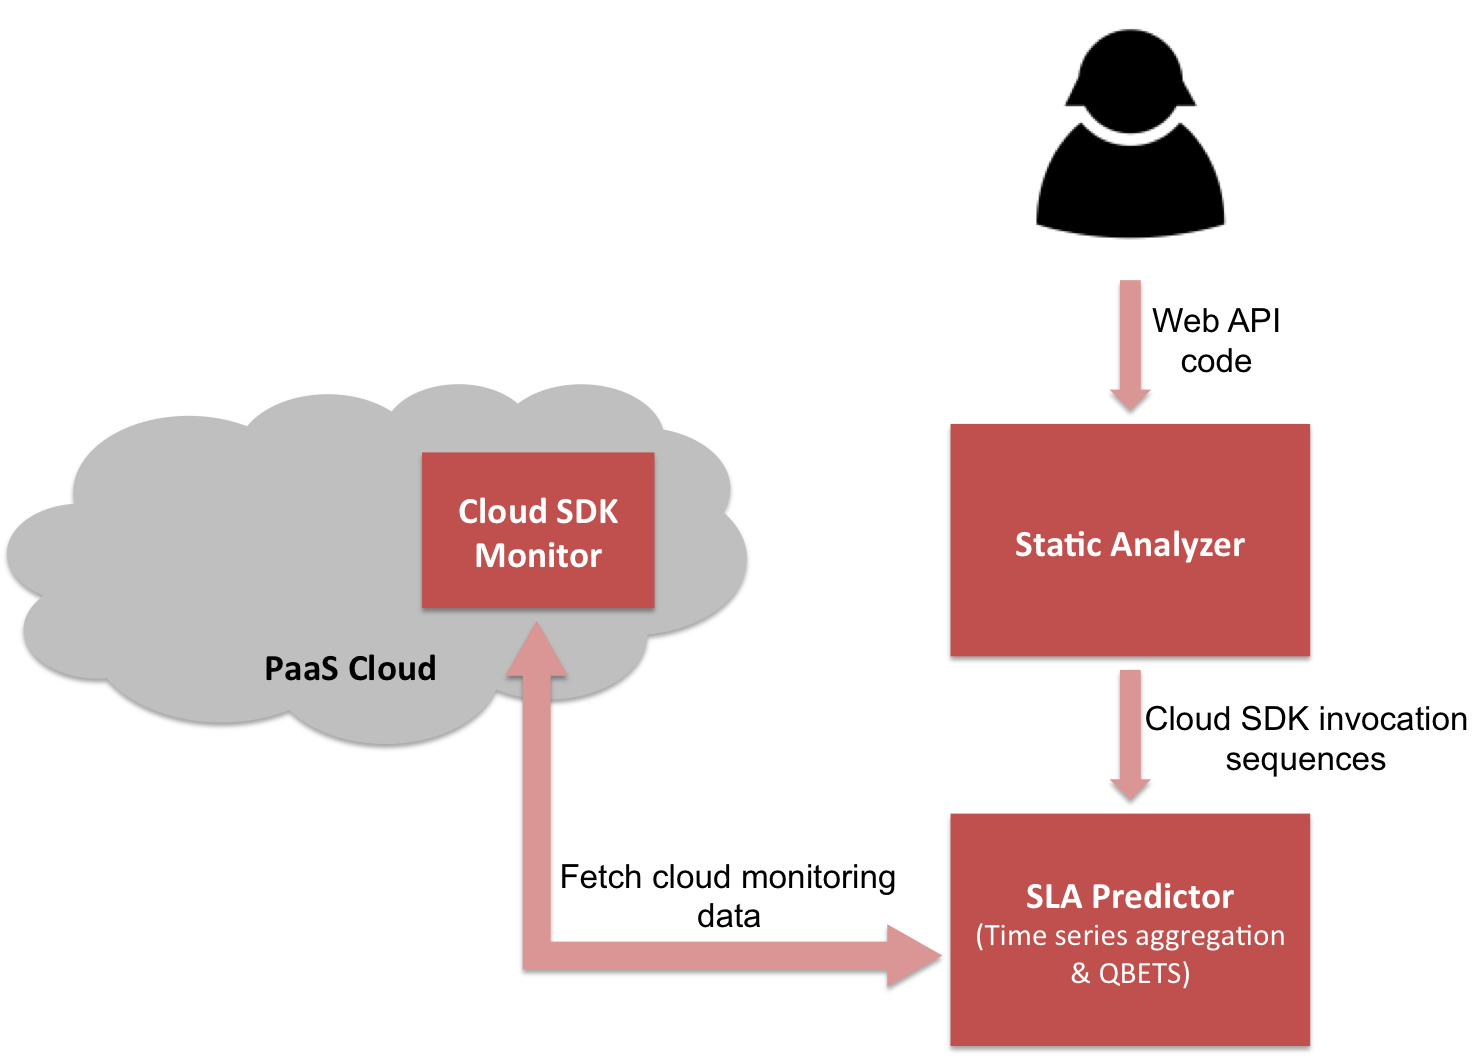
\includegraphics[scale=0.35]{cerebro_arch}
%\caption{Cerebro architecture and component interactions.}
%\label{fig:cerebro_arch}
%\end{figure}

%Additionally, we need a component that combines the results generated by above two components
%to make SLA predictions. Figure~\ref{fig:cerebro_arch} shows an overview of the resulting architecture.

\subsection{Static Analysis}
 This component analyzes the source code 
(or some intermediate representation of it), to identify
 the cloud SDK operations invoked by a given web API code. 
Since a web API code can only make a finite
 number of cloud SDK invocations, and since PaaS clouds only support a finite number of cloud
 SDK operations, it is possible to design an algorithm that
 extracts all cloud SDK invocations from any given web API code. 

Cerebro performs a simple construction and interprocedural static analysis 
of a method's control flow graph 
(CFG)~\cite{Allen:1970:CFA:800028.808479,Aho:1986:CPT:6448,Morgan:1998:BOC:288765,Muchnick:1998:ACD:286076} for each API method (externally facing) in a web API. 
The algorithm extracts all cloud SDK operations along
each path through the method.  Cerebro analyzes calls to other web API functions
that the method calls, recursively.  Cerebro caches cloud SDK details for each function 
once analyzed so that it can be reused efficiently for other call sites to the same
function. Cerebro does not analyze third-party library calls, if any.  Cerebro encodes
each cloud SDK call sequence for each path in a lookup table. Cloud SDK calls are 
easily identified by name, similarly to library calls.

To handle loops, we first extract them from the CFG and 
annotate any cloud SDK invocations that occur within them, in the cloud SDK sequence
for the path.  We annotate each with an estimate on the number of times
the loop is likely to execute in the worst case. We use a simple static
loop bounds estimator 
based on past work~\cite{bygde2010static,Gulwani:2009:CRP:1542476.1542518,Lokuciejewski:2009:FPS:1545006.1545064,Hunt:2006:PCL:1167999.1168026}
to enable this.  We perform cloud SDK operation annotation during CFG analysis
and estimate loop bounds separately afterward.

We have found (and show in our characterization of App Engine web APIs in the previous
section) that loops in these programs are rare and when they do occur, they are
used to iterate over a particular data set, commonly returned from the database.
For such data dependent loops, we estimate the bounds if specified 
in the cloud SDK call (e.g. the maximum number of 
entities to return~\cite{gae-fetch-options}).
If our analysis is unable to estimate the bounds for these loops, the tool asks
the developer for an estimate of the likely data set size.

\subsection{Platform Monitoring Agent: Watchtower}
Watchtower is the Cerebro component that tracks the performance of individual
cloud SDK operations within a PaaS system.  It is possible to implement
Watchtower as an integrated PaaS service or as a PaaS application (web API).
Watchtower runs in the background with but separate from other PaaS-hosted web APIs.
It performs cloud SDK operations on synthetic datasets and records timestamped response
times in the PaaS datastore on a operation basis.  Watchtower includes
benchmarks for loop iteration over datastore numbers of entities 
(i.e. iterative datastore reads)
that some App Engine web APIs employ.  
Watchtower periodically garbage collects old records to eliminate unnecessary storage.

The frequency with which
Watchtower collects data determines how often Cerebro 
is able to make SLA predictions for web APIs. Currently, we use a period of one minute
but this value is configurable.  Cerebro benchmarks iteratvie datastore reads
using 1, 1000, and 1000000 entities.  Cerebro monitoring is straightforward and
benchmarks can easily be added and customized to capture common PaaS-hosted web API
patterns.


\subsection{Making SLA Predictions}

To make SLA predictions, Cerebro uses 
Queue Bounds Estimation from Time Series (QBETS)~\cite{Nurmi:2007:QQB:1791551.1791556},
a non-parametric time series analysis method that we developed in prior work.
We originally designed QBETS for
predicting the scheduling delays for the batch queue systems 
used in high performance computing environments. 
We adapt it for use ``as-a-service'' in PaaS systems 
to predict the execution time of web APIs.

A QBETS analysis requires three inputs:
\begin{enumerate}
\item A time series of data generated by a continuous experiment,
\item The percentile for which an upper bound should be predicted ($p \in [1..99]$)
\item The upper confidence level of the prediction ($c \in (0,1)$)
\end{enumerate}

QBETS uses this information to predict an upper bound for 
the $p$-th percentile of the time series.
The predicted value has a probability of $0.01p$ of 
being greater than or equal to the next data point that
will be added to the time series by the continuous experiment. 
The upper confidence level $c$ serves as a conservative
bound on the predictions. That is, predictions made with an upper confidence 
level of $c$ will overestimate
the true percentile with a probability of $1-c$. This confidence guarantee 
is necessary because 
QBETS does not determine the 
percentiles of the time series precisely, but only estimates them. 

To further clarify what QBETS does, assume a continuous experiment 
that periodically measures the
response time of a web API. This results in a time series of 
response time data. Suppose at time $t$,
we run QBETS on the time series data collected so far 
with $p=95$ and $c=0.01$. The prediction returned
by QBETS has a 95\% chance of being greater than or equal 
to the next response time value measured
by our experiment after time $t$. Since $c=0.01$, the predicted value has a 99\% chance of
overestimating the true 95th percentile of the time series.

We find QBETS to be an ideal fit for our work due to several reasons. 
\begin{itemize}
\item QBETS works with time series data. Since
cloud SDK benchmarking data can be easily represented as time series,
they are highly amenable for QBETS analysis. 
\item QBETS makes predictions regarding the
future outcomes of an experiment by looking at the past 
outcomes -- an idea that aligns with our
goal of predicting future API response times from past cloud SDK benchmarking data. 
\item Response time
SLAs of web APIs should be specified with exact correctness 
probabilities and confidence levels for
them to be useful to developers and PaaS administrators. QBETS meets these requirements.
\item QBETS is 
simple, efficient and has been applied successfully to analyze a wide range of time series 
data, including correlated and uncorrelated data, in the past.
\end{itemize}

We now describe the Cerebro process.
Recall that our static analysis produces a list of annotated cloud SDK invocation sequences.
We start by pruning this list to eliminate duplicates. 
Duplicates occur when a web API code has
multiple paths of execution, where more than one path consists of the same sequence of cloud 
SDK invocations. Then for each sequence of cloud SDK 
invocations present in the pruned list, we
perform the following operations:

\begin{enumerate}
\item Retrieve benchmarking data from Watchtower 
for all operations in the sequence. Watchtower provides
this information as ordered time series data (one time series per cloud SDK operation).
\item Align all retrieved time series across operations and aggregate
to form a single time series for the sequence of cloud SDK operations.
\item Pass the aggregate time series to QBETS along with the 
desired $p$ and $c$ values to predict an
upper bound. 
\end{enumerate}

This process is exemplified as follows.
Suppose our static analysis results in the
cloud SDK invocation sequence $<op_{1},op_{2},op_{3}>$. 
Lets assume Watchtower has the following
time series data collected for the three operations in the sequence.

\begin{itemize}
\item $op_{1}$: $[t_{0}: 5, t_{1}: 4, t_{2}: 6, ...., t_{n}: 5]$
\item $op_{1}$: $[t_{0}: 22, t_{1}: 20, t_{2}: 21, ...., t_{n}: 21]$
\item $op_{1}$: $[t_{0}: 7, t_{1}: 7, t_{2}: 8, ...., t_{n}: 7]$
\end{itemize}

Here $t_{m}$ are timestamp values Watchtower has assigned to 
each data point. We align the three
time series, so that values with the same timestamp line up 
together, and aggregate the results
to obtain the following time series.

$[t_{0}: 34, t_{1}: 31, t_{2}: 35, ...., t_{n}: 33]$

Then we pass the aggregate time series to QBETS for analysis, and
treat the QBETS prediction as an SLA for the web API code.
If the QBETS predicted value is $Q$ milliseconds, 
we can form the SLA as ``the web API responds 
under $Q$ milliseconds, $p$ percent of the time''. 
When the code has multiple paths of execution (and
hence multiple sequences of cloud SDK operations), 
we predict more than one SLA for the API. In
such cases we treat the SLA with highest predicted value 
as the final SLA (i.e. the worst case SLA).

When the static analysis produces cloud SDK invocation 
sequences with information about loops, Cerebro performs an additional step.
If some operation has been tagged as being inside a loop, where the loop
bounds have been estimated, the time series data corresponding to that 
operation should be multiplied 
by the loop bound estimate, before aggregating. In cases where the operation 
is inside a data dependent loop, we request the time series data from a 
Watchtower iterative datastore read benchmark for a number of entities 
equal to or larger than the annotation. 

Another characteristic of QBETS is its warm up period.
QBETS requires a sufficiently large number of data points
in the input time series before it can make an accurate prediction. 
Specifically, we have proved that QBETS must to see 
at least $log(c)/log(0.01p)$ data points
before it can start making reliable predictions. 
This means, if we are interested in predicting the 95th percentile
of the API execution time, with an upper confidence of 0.01, 
Cerebro must feed QBETS with a time series that
contains at least 90 data points. We use this information to control 
Watchtower garbage collection.

\subsection{Cerebro Workflow}

%\begin{figure}
%\centering
%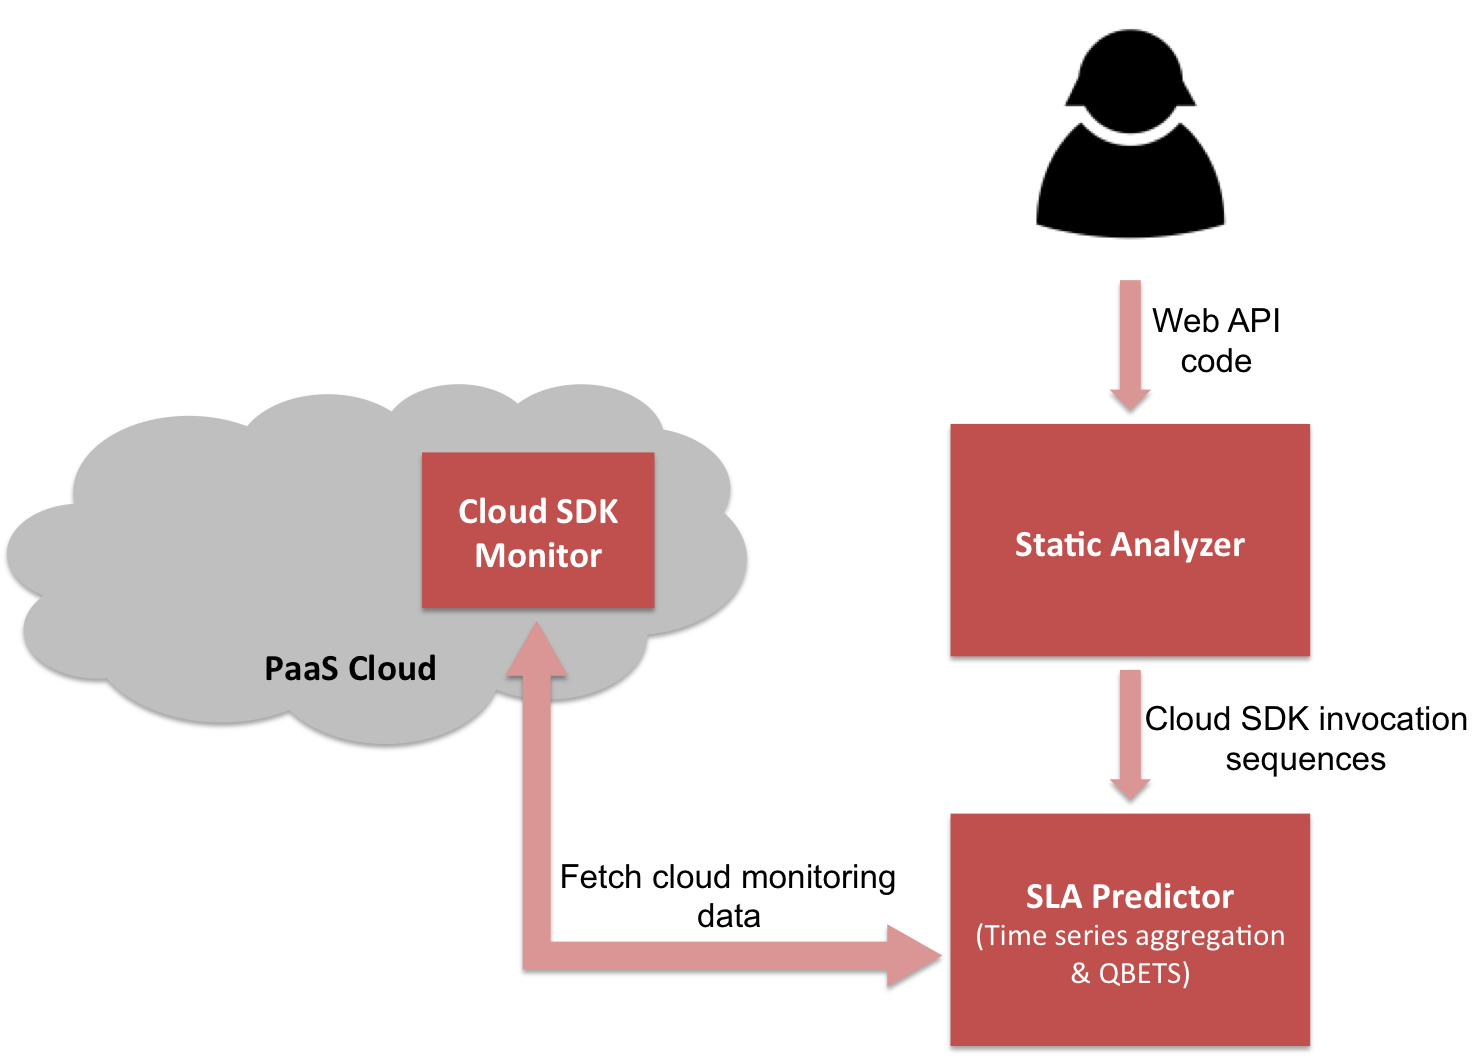
\includegraphics[scale=0.35]{cerebro_arch}
%\caption{Cerebro architecture and component interactions.}
%\label{fig:cerebro_arch}
%\end{figure}

Although we invoke Cerebro as part of the web API deployment process. Developers
can also do so during development using Cerebro's static analysis tool and interacting
with the Cerebro service in a PaaS cloud.
The static analyzer extracts the sequences of cloud SDK invocations from 
the web API code and passes them to Cerebro.
Cerebro contacts Watchtower 
to retrieve the relevant cloud SDK operation
benchmark data (time series) and aggregates them for QBETS processing.
Cerebro then generates a prediction using its QBETS service, which returns a prediction
for the percentile ($p$) and the upper confidence ($c$) values of interest.

The predictions can be used in many ways. In the simplest case they can be
used to clearly document the API SLAs, so that API consumers can stay informed about what 
type of performance to expect from the APIs they use. In a somewhat advanced context, 
Cerebro predictions can guide the API developers on how to program web APIs 
to support highly competitive SLAs. In an
more sophisticated environment, the Cerebro predictions can be used to 
enforce SLA-related policies on web APIs deployed in the cloud. Such an implementation
can run Cerebro on web APIs as they are submitted for deployment, 
and reject any APIs that do not
support the desired performance level.
